\section{Messung der Kennlinie des Verstärkers}

\subsection{Beschreibung}

In der letzten Messung soll die Kennlinie des Messverstärkers ermittelt
werden und damit der Verstärkungsfaktor $A$ bestimmt werden. Dafür liegt
eine Matrix mit den Eingangsspannungen $U_e$ und den Ausgangspannungen
$U_a$ vor.
Da der Verstärker Ausgangsseitig bei etwa $+13.75\mathrm{V}$ und 
$-13.06\mathrm{V}$ in Sättigung geht, werden die jeweils ersten 2
und die letzten beide Werte nicht betrachtet.

Die Steigung der linearen Funktion ist 

Der Verstärkungsfaktor $A$ ist der Quotient aus Ausgangs- und Eingangsspannung
und somit die Steigung.

\begin{equation} \label{eq141}
    \begin{split}
        A=\frac{U_a}{U_e}\simeq2 \mathrm{V}
    \end{split}
\end{equation}



\subsection{Ausgabe der Lösung}
\begin{figure}[H]
 \centering
 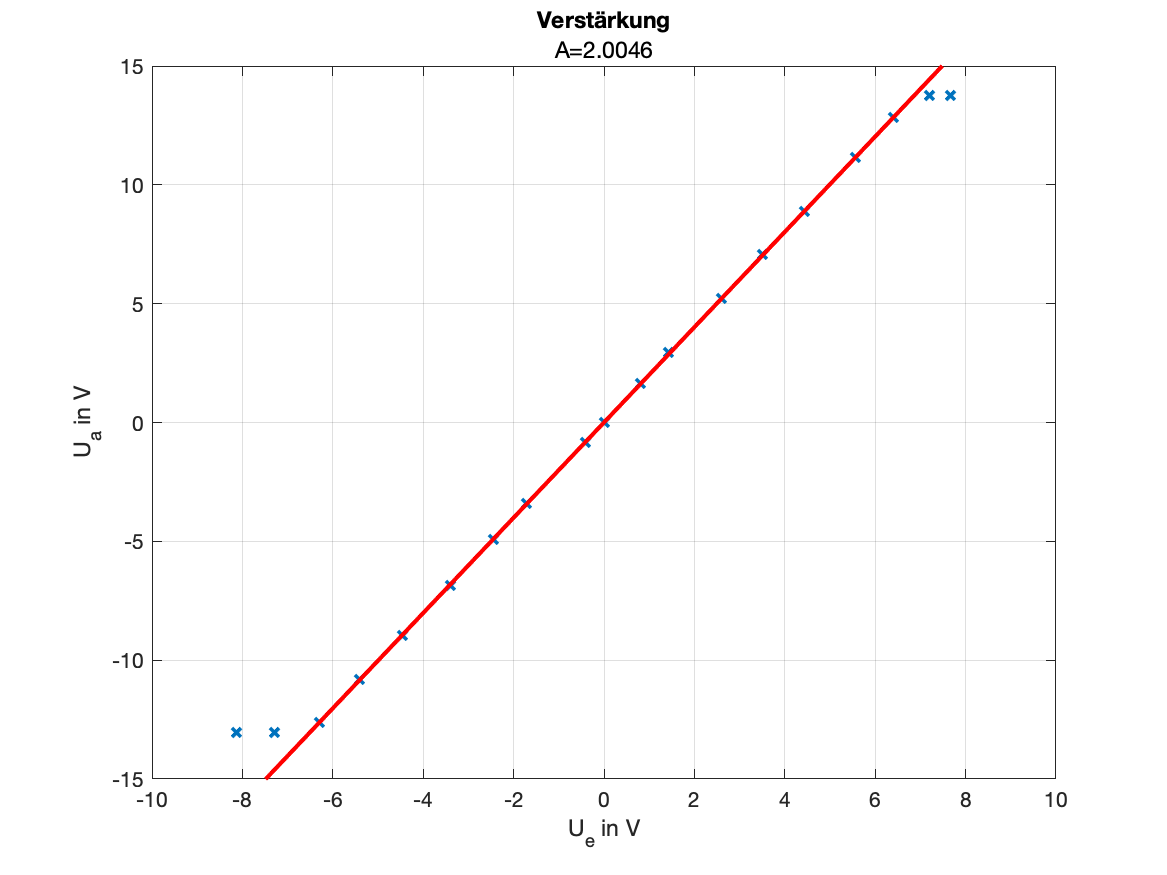
\includegraphics[width=1\textwidth]{as_labor01_4.png}
 \caption{Plot der Aufgabe 4}
 \label{fig:PlotAufgabe4}
\end{figure}

\subsection{Matlab Code}
\lstinputlisting[language=Matlab]{matlab/as_labor01_4.m}
